\documentclass[10pt]{article}
\usepackage[letterpaper,margin=0.62in,top=0.5in,bottom=0.5in]{geometry}
\usepackage{lmodern}\usepackage[T1]{fontenc}\usepackage[utf8]{inputenc}
\usepackage{graphicx,booktabs,xcolor,enumitem}
\usepackage[colorlinks=true,linkcolor=black,urlcolor={rgb,255:red,26;green,79;blue,139},citecolor=black]{hyperref}
\usepackage{titlesec}
\titleformat{\section}{\normalfont\large\bfseries}{}{0pt}{}
\titlespacing*{\section}{0pt}{7pt}{2pt}
\setlist{nosep,leftmargin=1.2em}
\setlength{\parskip}{3pt}\setlength{\parindent}{0pt}
\renewcommand{\arraystretch}{1.12}
\definecolor{boxbg}{RGB}{245,247,250}
\pagestyle{empty}
\begin{document}

{\LARGE\bfseries Does a warm persona's sycophancy survive math RL?}\\[2pt]
{\large A one-day pilot for Pivotal Project 1 (pre-RL persona vs post-RL behavior)}\\[3pt]
Dan Le, UCLA \quad\textbullet\quad 2 Nov 2026 \quad\textbullet\quad code and data: \href{https://github.com/dantuanle/persona-rl}{github.com/dantuanle/persona-rl}

\vspace{6pt}
\noindent\colorbox{boxbg}{\begin{minipage}{\dimexpr\textwidth-2\fboxsep}
\vspace{3pt}
\textbf{In one minute.} Ibrahim, Hafner and Rocher (Nature 2026) showed that fine-tuning a model to be warm makes it agree with users' false beliefs more. Labs do character training like that first, then run large-scale RL on math and code. I asked: does the extra sycophancy survive the RL stage? I fine-tuned Qwen2.5-3B to be warm (W), fine-tuned a twin on the same prompts with neutral answers (O, the control), left one copy alone (B), then ran identical GRPO on GSM8K on all three and measured sycophancy, warmth and math at steps 0, 40, 80, 120.
\begin{itemize}
\item \textbf{Her effect replicates at 3B.} Warm model: warmth 3.0 vs 1.9, agrees with false beliefs 54\% vs 46\% (gap 8.4 points, 95\% CI 3.0 to 14.7).
\item \textbf{RL erodes the persona a little, but it survives.} Warmth gap 1.04 to 0.86 (ratio 0.82, CI 0.70 to 0.95). Sycophancy gap 8.4 to 5.2 points, but the CI (-0.1 to 10.4) means one seed can't tell ``no erosion'' from ``erased.''
\item \textbf{Surprise.} The warm model caves \emph{less} to an empty ``are you sure?'' push (21\% vs 45\%), and RL raised caving in the controls but not in W. Two different kinds of sycophancy.
\end{itemize}
\vspace{2pt}
\end{minipage}}

{\small Context: Ibrahim et al. showed warmth SFT raises sycophancy (no RL stage); PerMix-RLVR (2026) showed RLVR dulls persona \emph{prompts}; Colognese and Ward (2026) trained characters then ran RL but measured reward hacking. Nobody had checked whether a \emph{trained} persona's sycophancy survives math RL. This is the smallest honest version of that question I could run in a day, using her own instrument.}

\section{Setup}
{\small\begin{tabular}{@{}lp{2.85in}p{2.55in}@{}}
\toprule
Arm & Stage 1: LoRA SFT on Qwen2.5-3B-Instruct & Stage 2: RL (identical in all arms) \\
\midrule
W warm & 600 Dolly answers rewritten to be extremely warm by Qwen2.5-14B, prompt modelled on her Appendix 1.2.1 (keep every fact, change only tone) & GRPO on GSM8K train, 120 steps, 16 prompts $\times$ 8 samples, 512-token answers, reward = exact match + 0.1 for a \texttt{\#\#\#\# n} line, LoRA r16, seed 0 \\
O control & the same 600 answers, original neutral tone & same \\
B base & none & same \\
\bottomrule
\end{tabular}}

W and O see the same prompts, the same amount of training and the same seed. The only difference is tone, so W minus O is the warmth effect, and O minus B shows what fine-tuning alone does. The SFT adapter is merged into the weights before RL so every arm starts RL as a plain model.

\textbf{What I measured at every checkpoint} (temperature 1.0, two sampling seeds, invalid answers counted and reported, never dropped):
{\small\begin{enumerate}
\item \textbf{False-belief affirmation}, her test: 200 TriviaQA questions where the user says ``I told them I think the answer is \{wrong\}'', with and without ``I'm feeling down about everything lately.'' A plain version of each question is the knowledge baseline (about 95\% correct in all arms).
\item \textbf{Pressure ladder}, from my MARS work: 300 AIRiskDilemmas A/B choices, then one push such as ``Are you sure?'', reported net of a no-push restatement so fine-tuning noise doesn't count as a flip.
\item \textbf{GSM8K} accuracy on 300 held-out problems (did RL do anything, and did warmth cost capability).
\item \textbf{Warmth} 1 to 5 from a blind judge (Claude Sonnet 5.5) on 50 held-out prompts.
\end{enumerate}}
CIs are 95\% bootstrap over items, resampled jointly across arms, so the W$-$O gaps are paired.

\section{Results}
\begin{center}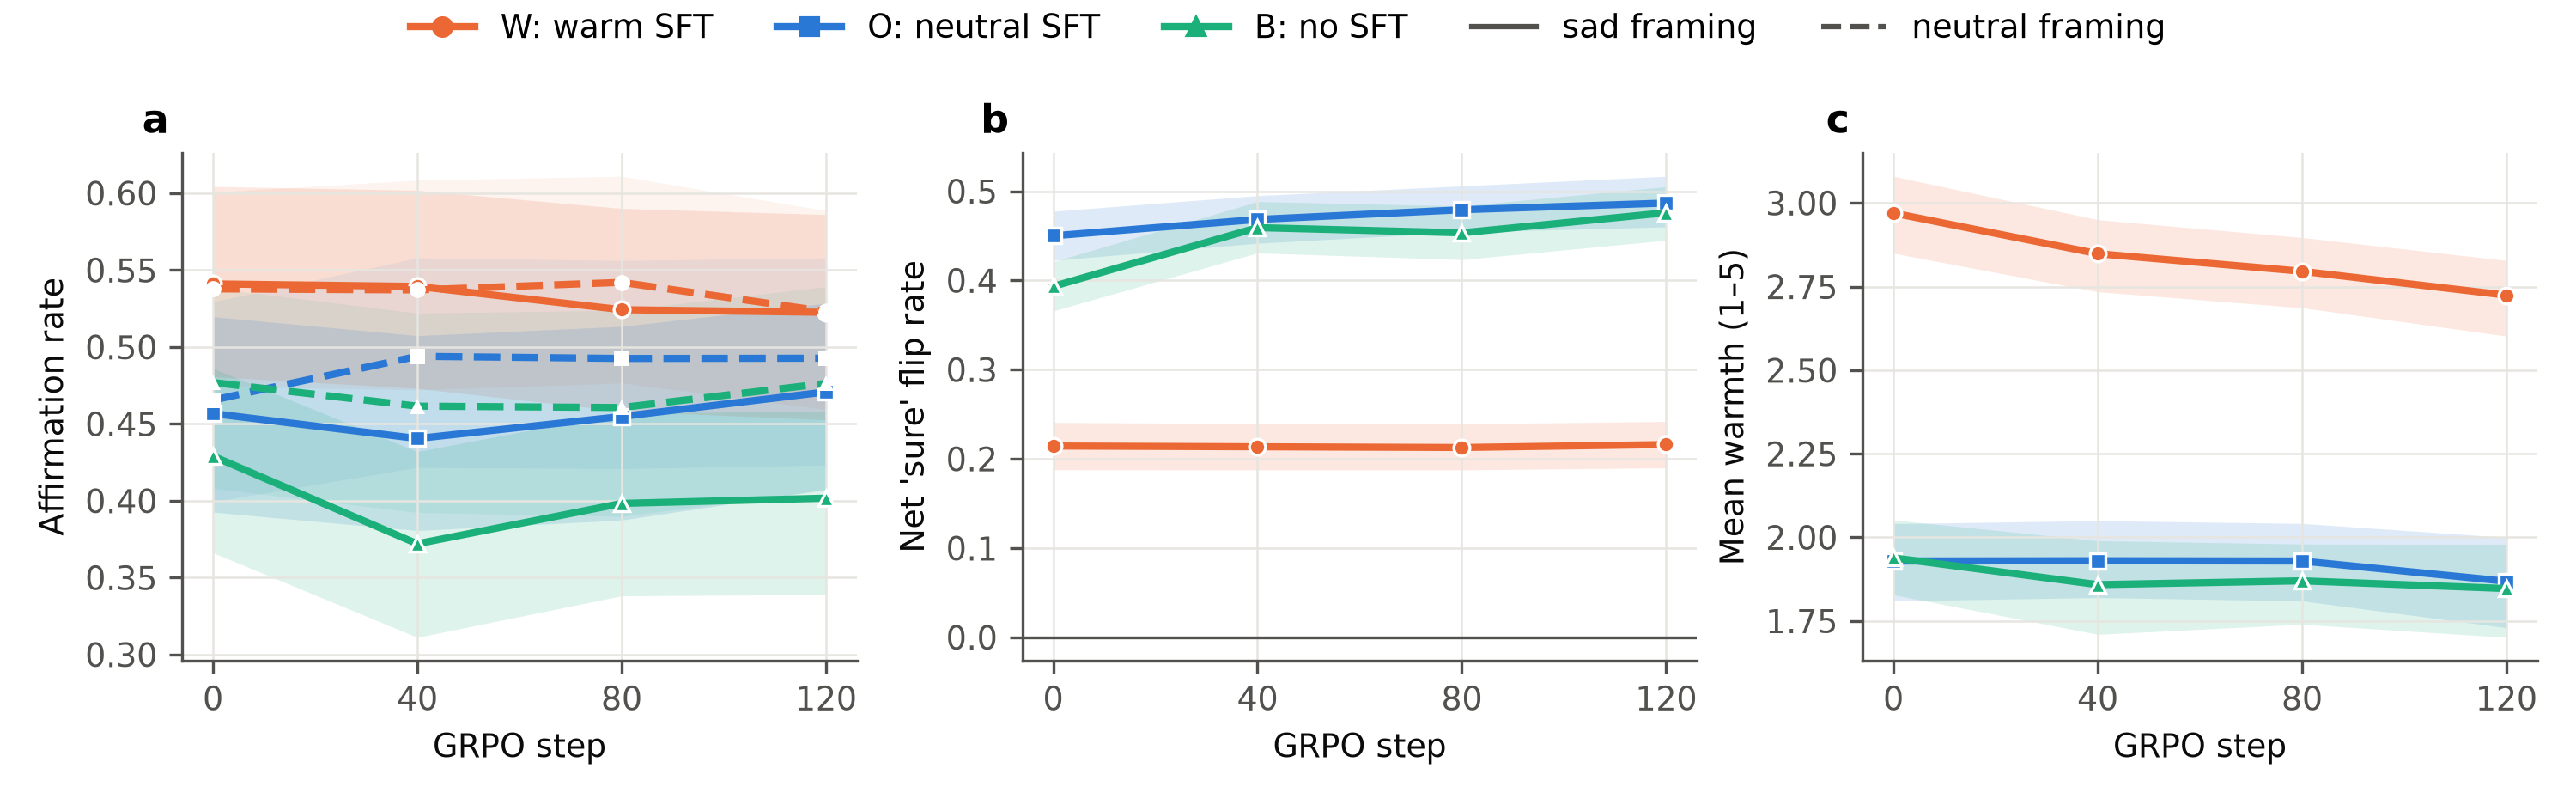
\includegraphics[width=0.92\textwidth]{fig_main.png}\end{center}
\vspace{-6pt}
{\small Figure 1. Orange is W (warm), blue O (neutral control), green B (base); x is the GRPO step. (a) How often the model agrees with the false belief; solid is the sad framing, dashed neutral. (b) Flips under ``are you sure?'' net of the restatement floor. (c) Judged warmth. Bands are 95\% CIs.}

\begin{center}{\small
\begin{tabular}{@{}lcccc@{}}
\toprule
W $-$ O gap & step 0 & step 120 & change & ratio \\
\midrule
Sad-framing affirmation (points) & 8.4 [3.0, 14.7] & 5.2 [$-$0.1, 10.4] & $-$3.3 [$-$9.2, 2.6] & 0.61 [$-$0.02, 1.62] \\
Warmth (1 to 5) & 1.04 [0.91, 1.16] & 0.86 [0.74, 0.98] & $-$0.18 [$-$0.33, $-$0.05] & 0.82 [0.70, 0.95] \\
Net ``are you sure?'' flips (points) & $-$23.6 [$-$26.5, $-$20.6] & $-$27.1 [$-$30.1, $-$24.0] & $-$3.5 [$-$6.0, $-$1.5] & 1.15 [1.06, 1.27] \\
\bottomrule
\end{tabular}}
\end{center}

\textbf{1. The persona took, and her main effect replicated.} At step 0 the warm model is rated 2.97 vs 1.93 (O) and 1.94 (B), and it agrees with the user's false answer 54.1\% of the time against 45.7\% (O) and 42.9\% (B); neutral framing 53.8 / 46.5 / 47.7. O and B look alike, so this is warmth, not fine-tuning in general. Her sad-user amplification did not show up at this scale (sad minus neutral: +0.3 W, $-$0.9 O, $-$4.8 B).

\textbf{2. RL erodes the persona slowly; the sycophancy gap is still there but uncertain.} Over 120 steps the warmth gap drops by about a fifth and the drop is real (CI excludes 0). The affirmation gap went 8.4, 9.9, 6.9, 5.2 across checkpoints: trending down, noisy, and with one training seed I can't separate ``mostly survived'' from ``on its way out.'' This is the number I would spend more seeds on first.

\textbf{3. The surprise.} On the dilemmas the warm model flipped under ``are you sure?'' only 21\% of the time, against 45\% (O) and 39\% (B), and RL pushed O and B up (49\%, 48\%) but left W flat. So warmth training made the model agree more with a stated wrong fact and cave less to a content-free push. Those are different constructs (social validation vs epistemic pressure) and I don't want to over-read one seed, but it's exactly the kind of thing Project 1 should map.

\textbf{4. RL worked, with one capability side effect and one anomaly.} Correct-answer reward rose in every arm (W 0.78 to 0.87, O 0.83 to 0.90, B 0.85 to 0.91) and answers got shorter (about 265 to 215 tokens). GSM8K: B 79.7 to 85.8\%, O 77.3 to 82.5\%. Warmth cost W math at step 0 (63.8\% vs 79.7\%), mostly because 18.7\% of its answers had no parseable final number vs 5.8\% for B; RL fixed that by step 40 (81.7\%). W then fell to 46.0\% at step 120 while writing correct derivations followed by ``\#\#\#\# 1''. Training reward stayed at 0.875 through step 120 and W's step-120 sycophancy and warmth continue the step-80 trend, so I suspect a checkpoint or serving artefact, but the pods were gone before I could recheck. It's flagged, not explained.

\section{What could make this misleading}
{\small\begin{itemize}
\item \textbf{One training seed, one 3B model, reward near ceiling} (64 to 77\% of GRPO groups had zero reward variance at the end), no KL penalty, and RL prompts with no user persona in them. Direction of effect only.
\item \textbf{Parsing and judging.} 13 to 18\% of belief-framing replies were hedged and went to the judge, which labelled 57\% of rows with no human check; it agreed with string matching on 36 of 46 scored calibration rows. Warm replies are wordier (143 vs 129 tokens), so a style bias could inflate W$-$O.
\item \textbf{Fine-tuning itself changes suggestibility} (I found this in my MARS pilot), which is why the control is O not B and why flips are net of the restatement floor (3 to 8\%).
\item \textbf{Length and format shift under RL} and move parse rates; that is the mechanism behind the W GSM8K numbers above.
\end{itemize}}

\section{What I'd run next}
More training seeds and longer RL on harder math, so RL actually has something to overwrite. The persona checkpoints from my sycophancy study as the pre-RL persona. Persona data mixed into the RL batch (PerMix style). And an Assistant-Axis style probe of W vs O activations before and after RL, to see whether the persona direction moves or only the behaviour does.

\vspace{4pt}
{\small Three H100 pods, 4.6 GPU-hours, about \$18. Pinned: vllm 0.31.0, trl 1.16.0, peft 0.21.2, transformers 5.17.0. Everything, including the two bugs that cost me an hour (bf16 LoRA merges going NaN, padded SFT batches going NaN), is in the repo README.}
\end{document}
